\documentclass[tikz, border=15pt]{standalone}
\usepackage{helvet}
\renewcommand{\familydefault}{\sfdefault}
\usetikzlibrary{arrows.meta, positioning, calc}

\begin{document}
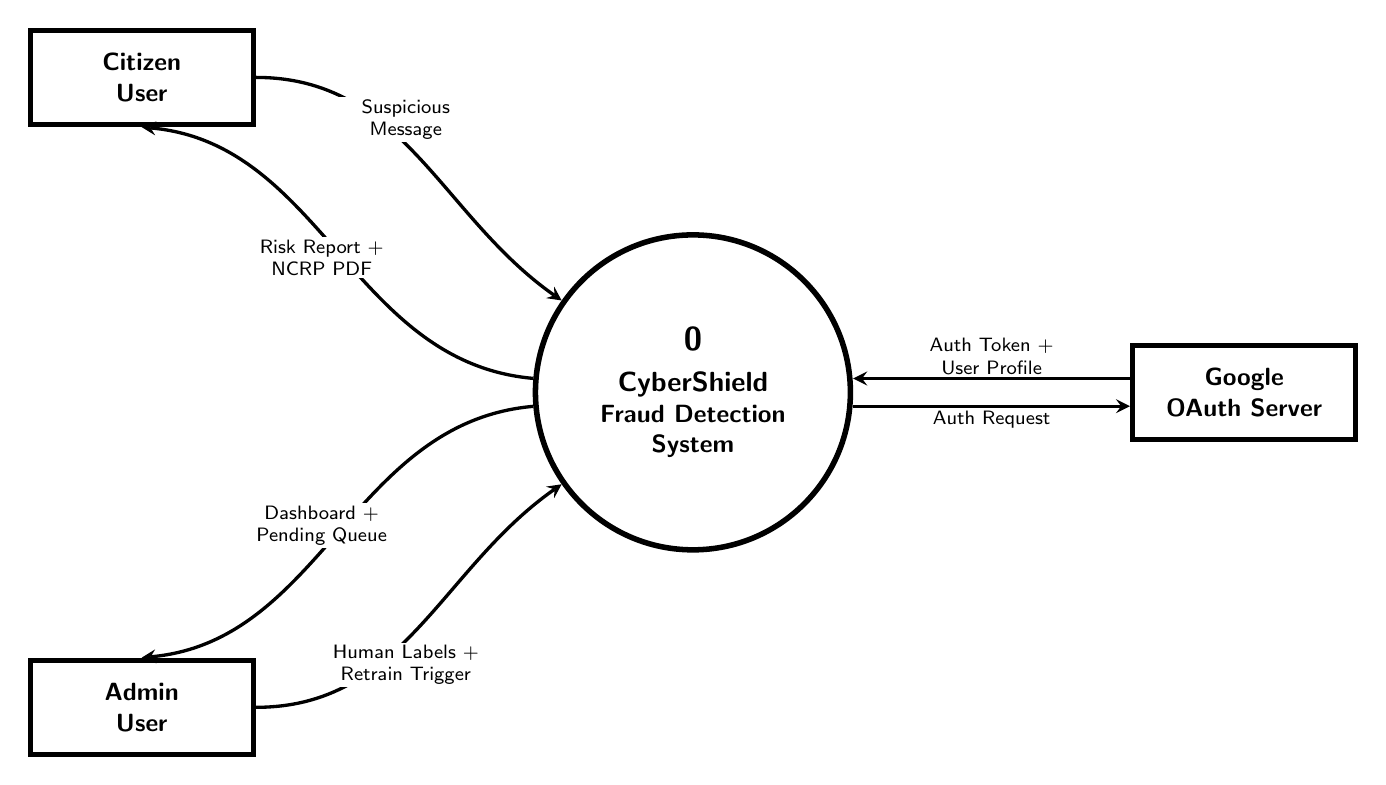
\begin{tikzpicture}[
    entity/.style={rectangle, draw=black, line width=1.8pt, fill=white,
        text width=2.6cm, align=center, minimum height=1.2cm, font=\small\bfseries},
    process/.style={circle, draw=black, line width=2pt, fill=white,
        minimum size=4cm, align=center, font=\small\bfseries},
    arr/.style={->, line width=1.2pt, >=stealth, draw=black},
    lbl/.style={font=\scriptsize, fill=white, inner sep=1pt,
                align=center, text width=2.2cm}
]

%% Central System
\node[process] (sys) at (0,0)
    {\large\textbf{0}\\[4pt]\normalsize CyberShield\\Fraud Detection\\System};

%% External Entities
\node[entity] (citizen) at (-7,  4)  {Citizen\\User};
\node[entity] (admin)   at (-7, -4)  {Admin\\User};
\node[entity] (oauth)   at ( 7,  0)  {Google\\OAuth Server};

%% ── Citizen → System (Suspicious Message) ────────────────────────
\draw[arr]
    (citizen.east)
    to[out=0, in=145]
    node[lbl, above, pos=0.45] {Suspicious\\Message}
    (sys.145);

%% ── System → Citizen (Risk Report + NCRP PDF) ───────────────────
\draw[arr]
    (sys.175)
    to[out=175, in=355]
    node[lbl, below, pos=0.55] {Risk Report +\\NCRP PDF}
    (citizen.south);

%% ── Admin → System (Labels + Retrain) ───────────────────────────
\draw[arr]
    (admin.east)
    to[out=0, in=215]
    node[lbl, below, pos=0.45] {Human Labels +\\Retrain Trigger}
    (sys.215);

%% ── System → Admin (Dashboard + Queue) ──────────────────────────
\draw[arr]
    (sys.185)
    to[out=185, in=5]
    node[lbl, above, pos=0.55] {Dashboard +\\Pending Queue}
    (admin.north);

%% ── OAuth → System: straight parallel lines ──────────────────────
\draw[arr]
    ([yshift=5pt]oauth.west) --
    node[lbl, above] {Auth Token +\\User Profile}
    ([yshift=5pt]sys.east);

\draw[arr]
    ([yshift=-5pt]sys.east) --
    node[lbl, below] {Auth Request}
    ([yshift=-5pt]oauth.west);

\end{tikzpicture}
\end{document}
